\subsection{Scene Objects and Meshes}
\label{sec:essential-concepts-scene-objects-and-meshes}

A scene object is represented as a \emph{mesh}, which is composed of a set of triangles, also known as \emph{primitives}, connected by their edges and vertices, as shown in Figure~\ref{fig:essential-concepts-mesh}.
Each object is identified by an index $o \in \NN_0$, and each primitive within an object is identified by an index $m \in \NN_0$.
Each primitive possesses three edges, identified locally by an index $\iota \in \{0, 1, 2\}$.
Primitives from different objects may share indices, therefore a primitive is uniquely identified by the pair $(o, m) \in \NN^2_0$.
Similarly, an edge is uniquely identified by the triplet $(o, m, \iota) \in \NN^3_0$.

\begin{figure}[ht!]
    \centering
    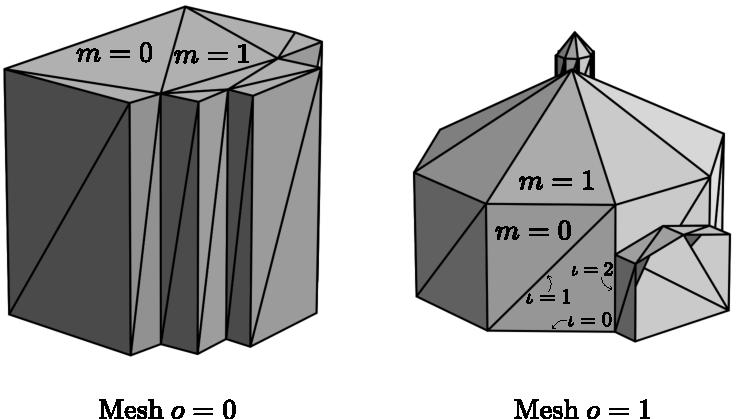
\includegraphics[width=0.6\textwidth]{figures/essential-concepts-mesh.pdf}
    \caption{A mesh is composed of triangular primitives connected by their edges and vertices. For clarity, only the indices of two primitives are displayed for each mesh. These meshes were downloaded from OpenStreetMap~\cite{OpenStreetMap} using Blosm~\cite{blosm}.\label{fig:essential-concepts-mesh}}
\end{figure}

\subsection{Rays and Paths}

A \emph{ray} $\LB \vv, \widehat{\kv}, t \RB$ is characterized by an origin $\vv \in \RR^3$, a direction $\widehat{\kv} \in \RR^3$, and a length $t \geq 0$. The direction $\widehat{\kv}$ is a unit vector, meaning $\norm{\widehat{\kv}} = 1$. If the length is unspecified, the ray is considered infinite, i.e. $t = \infty$. A \emph{path} $p^{(L)}$ with \emph{depth} $L \in \NN$ is a sequence of $L+1$ rays that connect a \emph{source} point $\sv \in \RR^3$ to a \emph{target} point $\tv \in \RR^3$, as illustrated in Figure~\ref{fig:essential-concepts-path},
\begin{equation}
    p^{(L)} = \LB \underbrace{\LB \vv^{(0)}, \widehat{\kv}^{(0)}, t^{(0)} \RB}_{\text{ray 0}}, \cdots, \underbrace{\LB \vv^{(L)}, \widehat{\kv}^{(L)}, t^{(L)} \RB}_{\text{ray $L$}} \RB
\end{equation}
where the superscript $(L)$ indicates the depth of the path, $\vv^{(0)} = \sv$, $\vv^{(i+1)} = \vv^{(i)} + t^{(i)} \widehat{\kv}^{(i)}$, and $\tv = \vv^{(L)} + t^{(L)} \widehat{\kv}^{(L)}$. The origins of the rays that form a path starting at the source and the target are known as the \emph{vertices} of the path. Hence, a path may be as well defined by a sequence of $L+2$ vertices:
\begin{equation}
    p^{(L)} = \left( \vv^{(0)} = \sv, \vv^{(1)}, \cdots, \vv^{(L)}, \vv^{(L+1)} = \tv \right)
\end{equation}
In this case, the rays have directions $\widehat{\kv}^{(i)} = \frac{\vv^{(i+1)} - \vv^{(i)}}{\norm{\vv^{(i+1)} - \vv^{(i)}}}$ and lengths $t^{(i)} = \norm{\vv^{(i+1)} - \vv^{(i)}}$ for $0 \leq i \leq L$.

\begin{figure}[ht!]
    \centering
    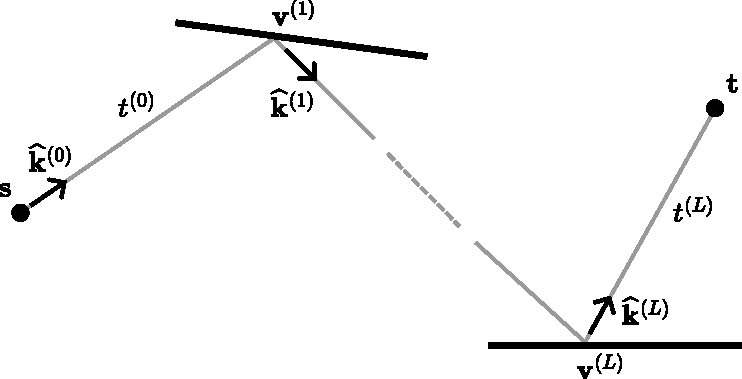
\includegraphics[width=0.50\textwidth]{figures/essential-concepts-path.pdf}
    \caption{A path consists of a sequence of ray segments connecting a source point $\sv$ to a target point $\tv$.\label{fig:essential-concepts-path}}
\end{figure}

The \emph{suffix} of a path, denoted by $p^{(\ell:)}$ where $0 \leq \ell \leq L$, is defined as the sub-path consisting of all the rays from the $\ell$-th one onward, i.e.
\begin{equation}
    p^{(\ell:)} = \left( \left(\vv^{(\ell)}, \widehat{\kv}^{(\ell)}, t^{(\ell)}\right), \cdots, \left(\vv^{(L)}, \widehat{\kv}^{(L)}, t^{(L)}\right) \right).
\end{equation}
Similarly, the corresponding \emph{prefix} is:
\begin{equation}
    p^{(:\ell)} = \left( \left(\vv^{(0)}, \widehat{\kv}^{(0)}, t^{(0)}\right), \cdots, \left(\vv^{(\ell-1)}, \widehat{\kv}^{(\ell-1)}, t^{(\ell-1)}\right) \right).
\end{equation}

\subsection{Interactions with Scene Objects}

\SRT{} currently supports four types of interactions with scene objects:
\begin{description}
    \item[Specular reflection ($\Rc$):] The wave is reflected with a reflection angle equal to the incident angle, as illustrated in Figure~\ref{fig:path-solver-ref}.
    \item[Diffuse reflection ($\Sc$):] The wave is reflected in multiple directions, as illustrated in Figure~\ref{fig:path-solver-ref}.
    \item[Refraction ($\Tc$):] The wave propagates into the scattering medium. The solvers assume that object surfaces are thin enough that their effect on transmitted rays (i.e. rays that traverse the surfaces through double refraction) can be modeled by a single transmitted ray. The transmitted rays are traced without angular deflection. Surfaces like walls should be modeled as single flat surfaces, as illustrated in Figure~\ref{fig:path-solver-trans-model}.
    However, when computing the transmitted and reflected fields, the thickness of the traversed object is considered.
    \item[Diffraction ($\Dc$):] The wave encounters a wedge-shaped object and is diffracted, as shown in Figure~\ref{fig:path-solver-diffraction-model}. Diffraction occurs in all directions along the \emph{Keller cone}~\cite{Keller:62}, where the angle between the incident ray and the wedge edge, denoted by $\beta_0'$, equals the angle between the diffracted ray and the wedge edge, denoted by $\beta_0$. The wedge exterior angle is denoted by $n\pi$, such that $n \in [1, 2]$. If the wedge's exterior angle $n\pi$ equals $2\pi$, i.e., $n = 2$, the wedge is termed an \emph{edge}.
\end{description}
The set of possible interaction types is denoted by $\Ic = \{\Rc, \Sc, \Tc\, \Dc\}$.

\begin{figure}[ht!]
    \centering
    \begin{subfigure}[b]{0.4\textwidth}
        \centering
        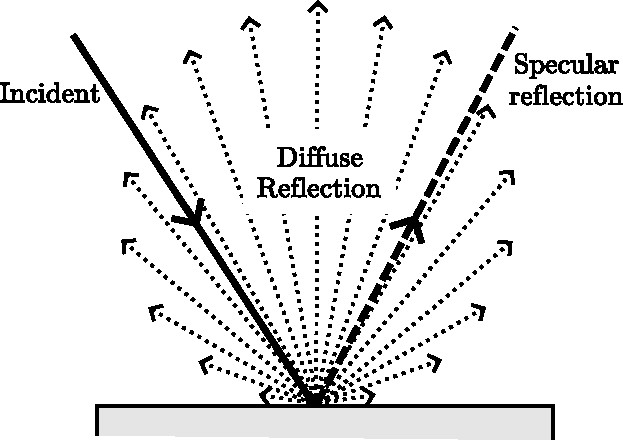
\includegraphics[width=\textwidth]{figures/path-solver-ref.pdf}
        \caption{Specular (dashed line) and diffuse reflection (dotted lines). Inspired by a figure from~\cite{Wikipedia-Diffuse-Reflection}.\label{fig:path-solver-ref}}
    \end{subfigure}
    \hfill
    \begin{subfigure}[b]{0.4\textwidth}
        \centering
        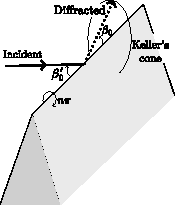
\includegraphics[width=0.65\textwidth]{figures/diffraction_wedge_3d.pdf}
        \caption{Diffraction of an incident wave by a wedge-shaped object.\label{fig:path-solver-diffraction-model}}
    \end{subfigure}
    \vspace{1em}

    \begin{subfigure}[b]{\textwidth}
        \centering
        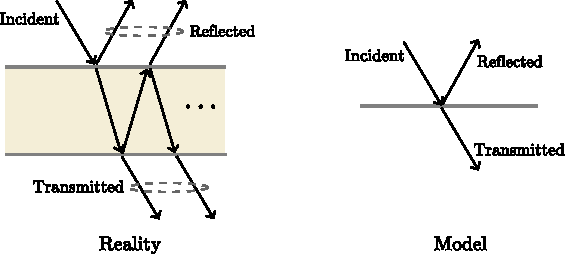
\includegraphics[width=0.6\textwidth]{figures/path-solver-transmission-reality.pdf}
        \caption{Transmission model.\label{fig:path-solver-trans-model}}
    \end{subfigure}
    \caption{\SRT{} currently supports specular reflection, diffuse reflection, refraction, and diffraction.}
\end{figure}

\subsection{Ray Tubes}
\label{sec:essential-concepts-ray-tube}

While a more detailed background on the propagation of \gls{EM} waves is provided in Appendix~\ref{sec:primer-em}, we introduce here some essential \gls{EM} concepts that are required for understanding the process of ray tracing. The source $\sv$ is modeled as a \emph{point source}, an infinitesimally small emitter of \gls{EM} waves that radiates in all directions according to a user-defined \emph{transmitter antenna pattern}.
Note that modeling transmit antennas as point sources is a valid approximation when the distances to scatterers and targets are significantly greater than the wavelength of the propagating waves.
Each ray traced from the source $\sv$ serves as the axial ray of a \emph{ray tube}~\cite[Chapter~2]{McNamara90}, which is a bundle of rays adjacent to the axial one. These ray tubes originate at the source and have a length $r$ and an angular opening $\omega$, as illustrated in Figure~\ref{fig:essential-ray-tube}. Importantly, specular reflection and refraction through planar surfaces only alter the ray direction. Diffuse reflection and diffraction alter the shape of the wavefront. As detailed in Sections~\ref{sec:path-solver} and~\ref{sec:radio-map-solver}, this process requires specific computations to determine the path vertices and corresponding fields. For a given path $p^{(L)}$ with depth $L$, we denote by $\boldsymbol{\chi}^{(L)} = \left(\chi^{(1)}, \cdots, \chi^{(L)}\right) \in \Ic^L$ the sequence of interaction types along the path. A key quantity for the remainder of this document is the depth of the last diffuse reflection or diffraction, denoted by $\ell_d \in \NN$ and defined as:
\begin{equation}
    \label{eq:essential-concepts-ell_d}
    \ell_d =
    \begin{cases}
        \max_{\substack{1 \leq \ell \leq L}} \left\{ \ell~:~\chi^{(\ell)} = \Sc \right\} & \text{ if } \exists \ell : \chi^{(\ell)} = \Sc \\
        0 & \text{ otherwise.}
    \end{cases}
\end{equation}
The dependency of $\ell_d$ on $\boldsymbol{\chi}^{(L)}$ is omitted for brevity. The case where $\ell_d = 0$ corresponds to paths that do not contain any diffuse reflection, known as \emph{specular chains}. If $\ell_d > 0$, then the suffix $p^{(\ell_d:)}$ is referred to as the \emph{specular suffix} of $p$. The value $\ell_d$ represents the depth index from which the path is composed solely of specular reflections, refractions, and diffraction, and is termed the \emph{specular suffix index} of $p$.

\begin{figure}[ht!]
    \centering
    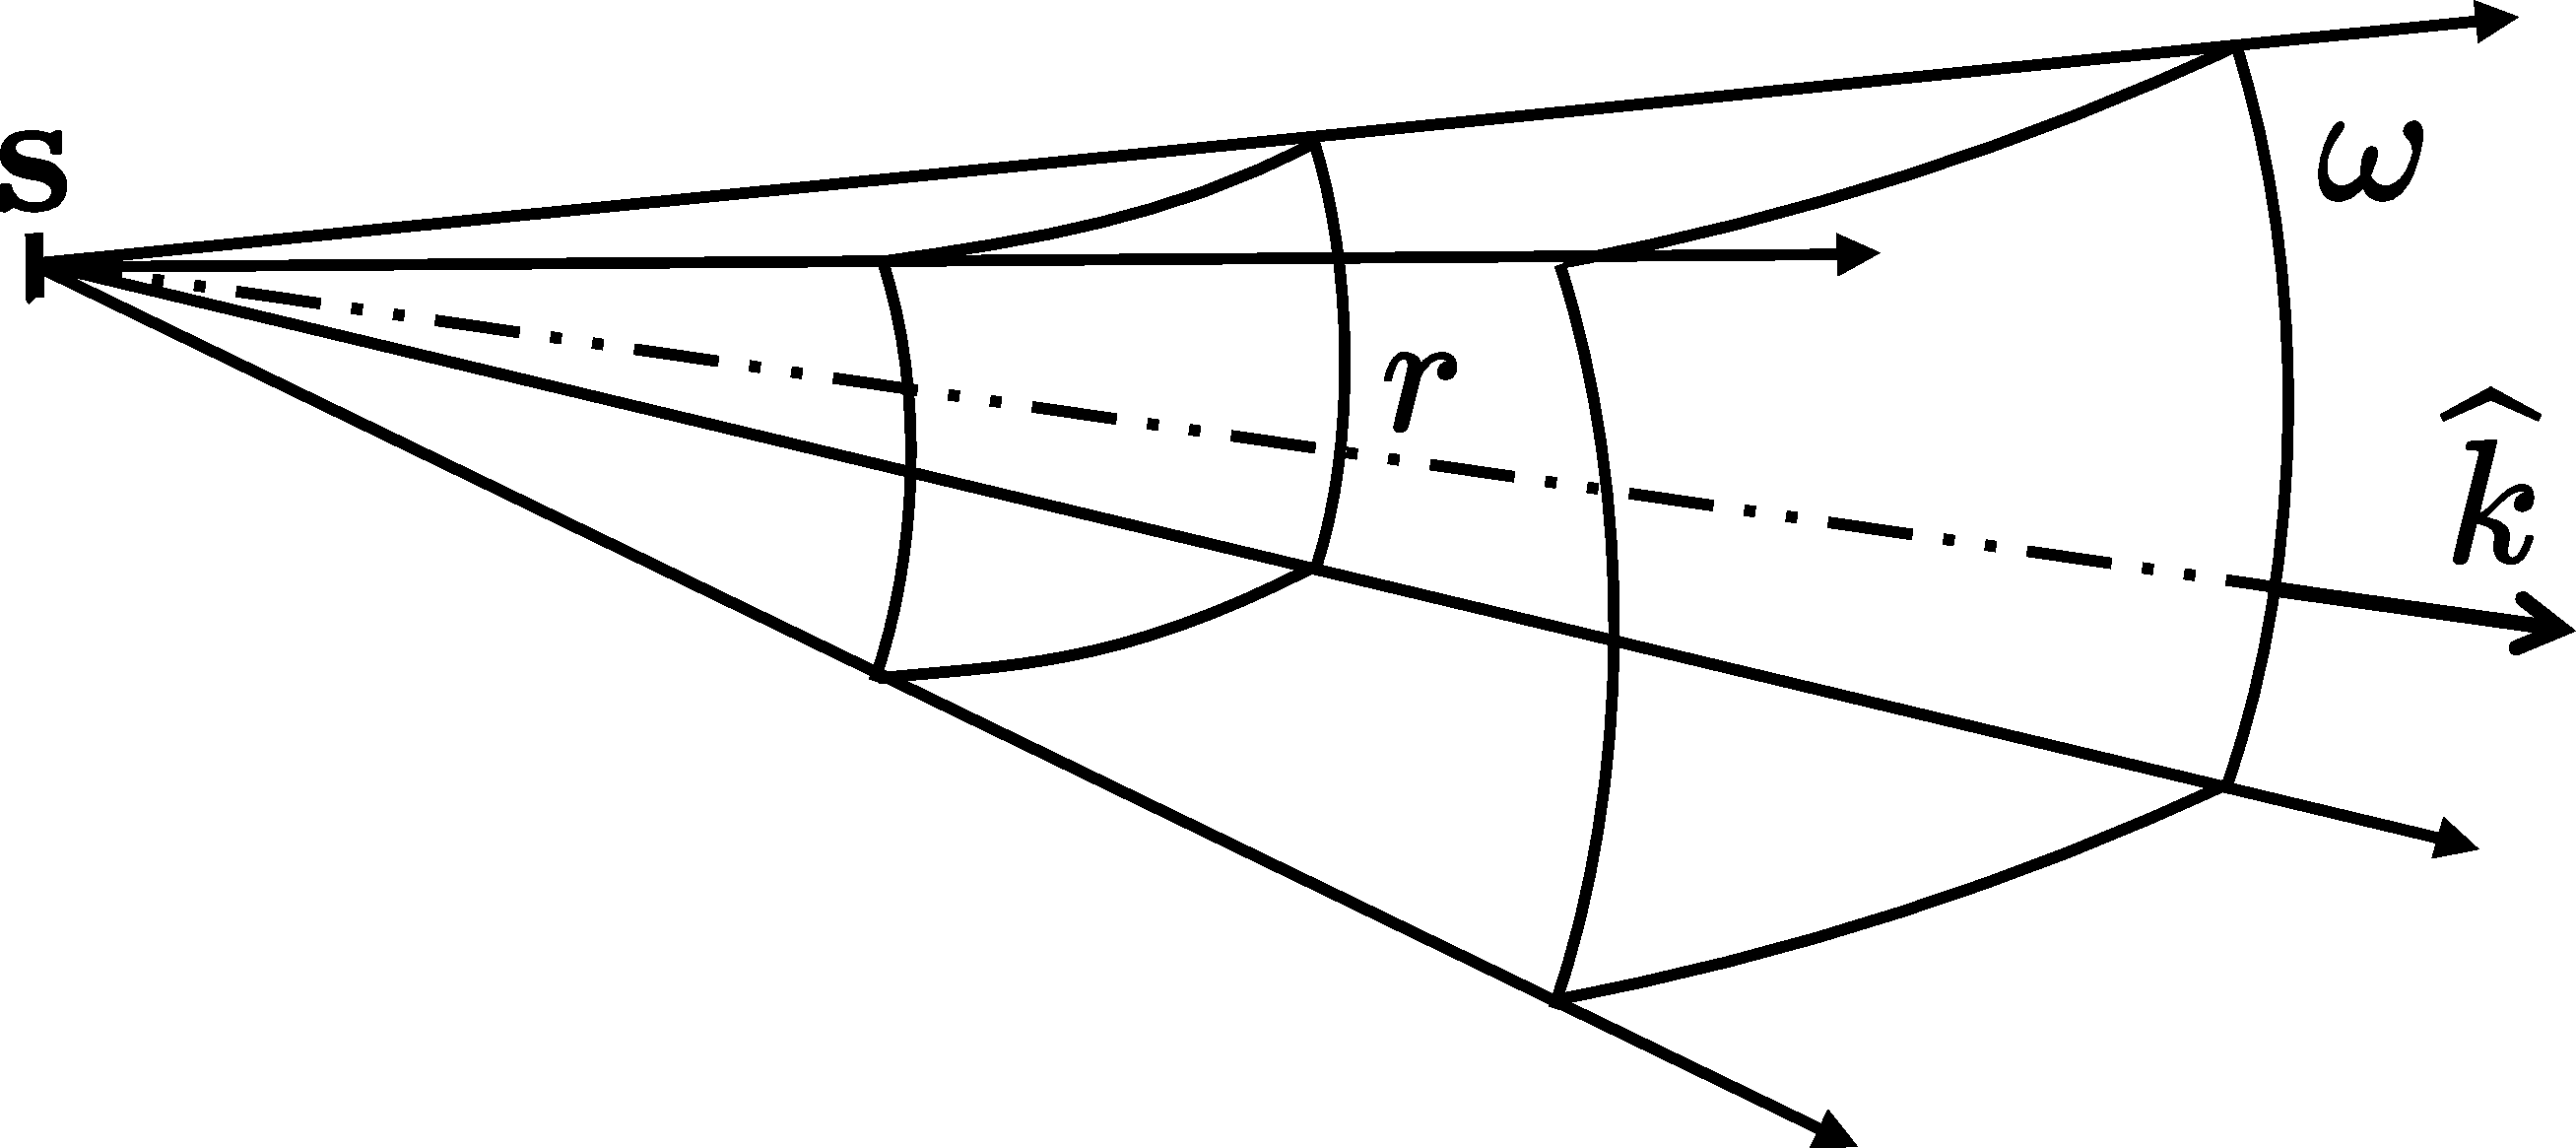
\includegraphics[width=0.4\textwidth]{figures/essential-concepts-ray-tube.pdf}
    \caption{A ray tube is a bundle of rays adjacent to an axial ray.\label{fig:essential-ray-tube}}
\end{figure}
